% * Week 2. (Aug 3) Business Analytics and Statistical Learning. Ch2. (Rob & Souhaib)
%   - Lecture 3: More on R and statistical learning. 
%   - Lab 2: 
%   - Lecture 4: Assessing model accuracy. Bias-variance tradeoff

%   Content: 
%     - Statistics? Machine learning? data mining? data science? Analytics? 
%     - The four V’s of big data/data science
%     - Analytics and data science jobs: “By 2018, the US could face a shortage of up to 190.000 workers with analytical skills” McKinsey


\documentclass[14pt]{beamer}
\usepackage{pgf,tikz,pgfpages,amsmath,bm,fancyvrb,animate}
\usepackage{graphicx,bera,booktabs}
\usepackage[australian]{babel}
\usepackage[utf8]{inputenc}

\usetheme{Monash}
\def\biz{\begin{itemize}[<+-| alert@+>]}
\def\eiz{\end{itemize}}
\def\ben{\begin{enumerate}[<+-| alert@+>]}
\def\een{\end{enumerate}}

\graphicspath{{../figures/}{../figures/book_figures/Chapter5/}}


\title[4. The Bootstrap]{Business Analytics}
\author{Week 4\\ The Bootstrap}
\date{20 August 2015}

\DefineShortVerb{\"}
\def\FancyVerbFormatCom{\color[rgb]{0.6,0,1}\relax}


\begin{document}

\begin{frame}[plain]{}
\maketitle
\begin{textblock}{11}(0.5,1.3){\color{white}\large
\textbf{ETC3250}}
\end{textblock}
\end{frame}

\begin{frame}{\large Pull yourself up by your bootstraps}
\fullheight{Bootstraps}
\end{frame}


\begin{frame}[plain]{What is the bootstrap?}
%
The bootstrap is a flexible statistical tool to \textbf{quantify the uncertainty} associated with a \emph{given estimator} or \emph{statistical learning method}.
\begin{center}
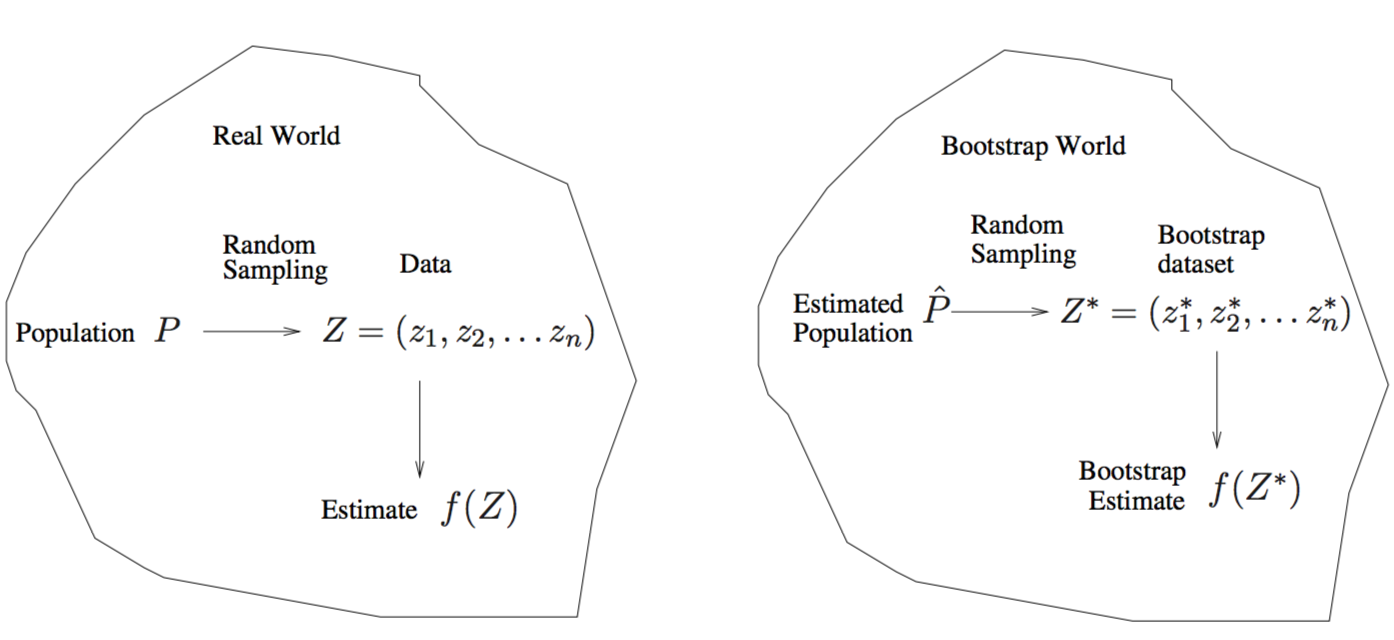
\includegraphics[width=1\textwidth]{general-bootstrap}	
\end{center}
\end{frame}

\begin{frame}[plain]{What is the bootstrap?}

\begin{itemize}
	\item  The bootstrap allows us to use a computer to \textbf{mimic the process of obtaining new data sets}, so that we can estimate the variability of our estimate without generating additional samples
	\item Rather than repeatedly obtaining independent data sets
from the population, we instead obtain distinct data sets (with the same size as our original dataset) by repeatedly sampling observations \textbf{from the original data set with replacement} (nonparametric) or \textbf{from an estimated model} (parametric).
\end{itemize}
\end{frame}

\begin{frame}[plain]{Illustration of the bootstrap}

\begin{center}
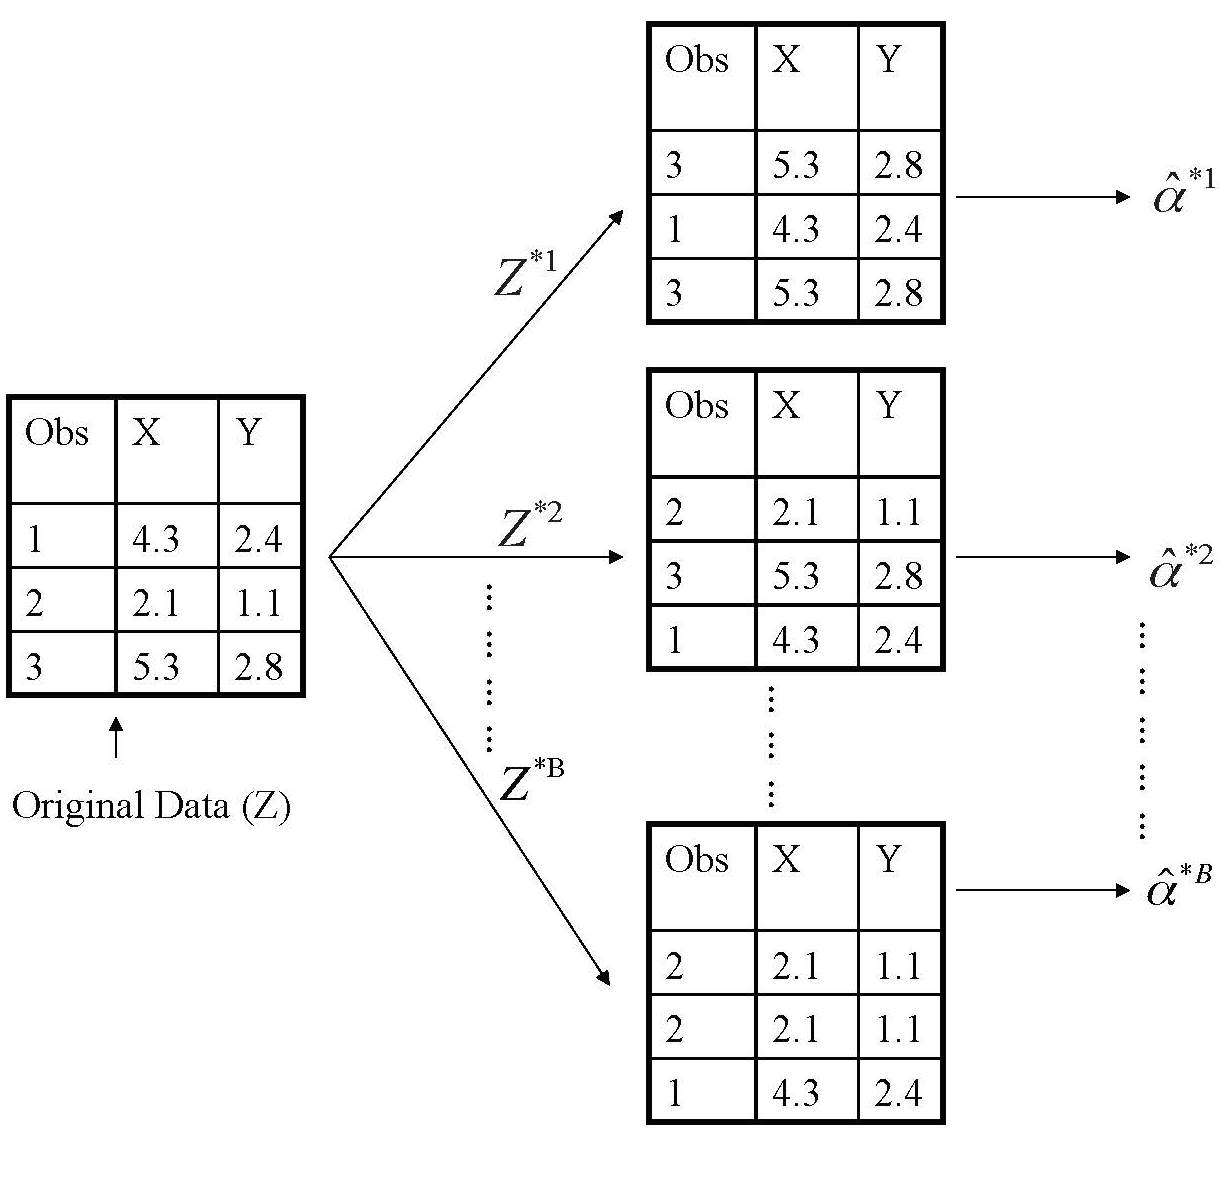
\includegraphics[width=.7\textwidth]{5-11.png}	
\end{center}
\end{frame}

\begin{frame}[plain]{The bootstrap procedure}
\begin{itemize}
	\item Find a good estimate $\hat P$ of $P$
	\begin{itemize}
		\item Parametric bootstrap
		\item Nonparametric bootstrap
	\end{itemize}
	\item Draw $B$ independent bootstrap samples $X^{*(1)}, \dots, X^{*(B)}$ from $\hat P$:

	$$X_1^{*(b)}, \dots, X_n^{*(b)} \sim \hat P \quad b = 1, \dots, B.$$ 	
	
	\item Evaluate the bootstrap replications:
 
		$$\hat \theta^{*(b)} = s(X^{*(b)}) \quad b = 1, \dots, B.$$	

	\item Estimate the quantity of interest from the simulated distribution of the $\hat \theta^{*(b)}$
\end{itemize}
\end{frame}

\begin{frame}[plain]{Examples}

What is the standard error of $\hat\theta$ (i.e., the standard deviation of the sampling distribution of $\hat \theta$)?

\begin{enumerate}
	\item $\hat \theta = \text{sample mean}$ 

	\item $\hat \theta = \text{sample median}$

\item $\hat\theta = $ expected shortfall at 5\%

\item $\hat\theta=$ lag 1 autocorrelation.
\end{enumerate}



\end{frame}



\begin{frame}[plain]{Prediction error estimation}

\begin{itemize}
	\item Fit the model on a set of bootstrap samples, and then keep track of how well it predicts the original training set
	
	$$ \text{Err}_{\text{boot}} = \frac1B \frac1N \sum_{b = 1}^B \sum_{i = 1}^N L(y_i, \hat f^{*b}(x_i))$$ 
	\pause
	\item Each of these bootstrap data sets is created by sampling with replacement, and is the same size as our original dataset. As a result some observations may appear more than once in a given bootstrap data set and some not at all.
\end{itemize}

\end{frame}

\begin{frame}[plain]{Prediction error estimation}
%

\begin{itemize}
	\item Training and validation sets have observations in common! Overfit predictions will look very good.
	
	
\begin{align*}
	&\text{P}(\text{observation~} i \in \text{~bootstrap sample~} b) \\
	&= 1 - (1 - \frac1n)^n \\
	&\approx 1 - \frac1e \\
	&= 0.632
\end{align*}
	
	\item Remember that cross-validation uses \emph{non-overlapping} data for the training and validation samples
\end{itemize}



\end{frame}


\begin{frame}[plain]{Prediction error estimation}

Better bootstrap version: we only keep track of predictions from bootstrap samples not containing that observation. The leave-one-out bootstrap estimate of prediction error can be defined as
\[ 
\text{Err}_{\text{loo-boot}} = \frac1N \sum_{i = 1}^N \frac{1}{|C^{-i}|}\sum_{b \in C^{-i}} \ L(y_i, \hat f^{*b}(x_i))
\]
where $C^{-i}$ is the set of indices of the bootstrap samples $b$ that do not contain observation $i$.\\

Problem of overfitting with $\text{Err}_{\text{boot}}$ solved but training-set-size bias as with cross-validation.

\end{frame}

% 	\item Other bootstrap procedures: bootstrap for time series, bagging, etc.
\begin{frame}[plain]{Many applications}

\begin{itemize}
	\item Computing standard errors for complex statistics
	\item Prediction error estimation
	\item Bagging (Bootstrap aggregating)
	\item ...
\end{itemize}	
\pause

\begin{block}{Variations}
There are several types of bootstrap based on different assumptions:
\begin{itemize}\itemsep=0cm\parskip=0cm
\item block bootstrap
\item sieve bootstrap
\item smooth bootstrap
\item residual bootstrap
\item wild bootstrap
\end{itemize}
\end{block}
\end{frame}





\end{document}